\section{Approach Overview}
\label{sec:overview}


\begin{figure*}[t]
\begin{center}
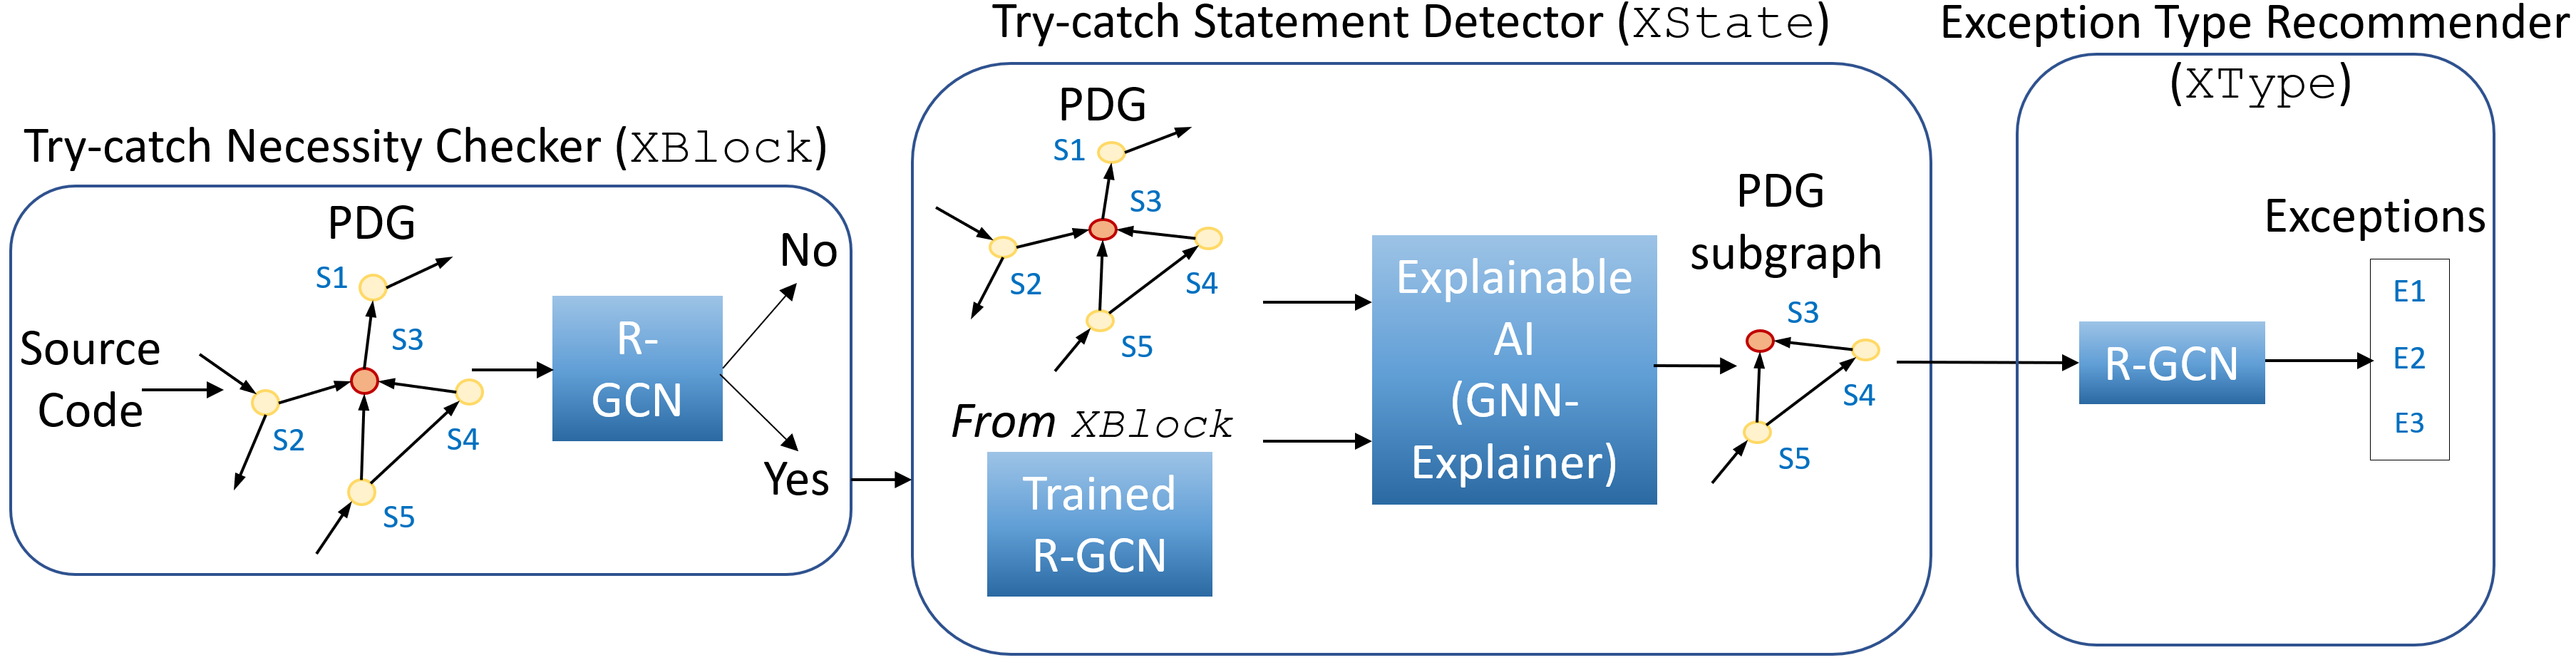
\includegraphics[width=5.4in]{overview.png}
\vspace{-10pt}
\caption{{\tool}: Architecture Overview}
\label{overview}
\end{center}
\end{figure*}

Let us present the overview of our approach. In general, {\tool}
consists of three main components. The first component called
{\xblock} aims to check if it is neccessary to have a \code{try-catch}
block for the given code snippet $C$. We extract the program dependence
graph (PDG) from the source code using DeepPDA~\cite{icse23} that is
capable of generating the PDG for any (in)complete code
snippet. The PDG is used an input for a Relational Graph Convolutional
Network (R-GCN)~\cite{yi}. During training, we use the complete source
code in the open-source projects in which each positive sample
contains at least a \code{try-catch} block, and each negative one does
not. If there are multiple consecutive blocks, we split them into
individual ones. During prediction, {\xblock} uses the trained R-GCN
to predict whether the given source code needs a \code{try-catch}
block or not.

In the case of the code snippet $C$ needs a \code{try-catch} block,
the second component, {\xstate}, is aimed to detect which statements
in $C$ that need to be placed within the \code{try-catch} block.
{\xstate} takes two inputs: 1) the PDG of the given code snippet, and
2) the trained R-GCN model for the \code{try-catch} necessity checker
({\xblock}). {\xstate} leverages the Graph-based Explainable AI model
named GNNExplainer~\cite{tien} to determine the statements in the PDG
that are most decisive and relevant to the reason why the snippet $C$
is required to have a \code{try-catch} block. The output of this
component is a list of statements in $C$ (e.g., $S_3$, $S_4$, $S_5$).
During training, ...
